% !TeX spellcheck = en_US
\documentclass[french]{yLectureNote}

\title{Atomistique 2 - PS}
\subtitle{Chimie}
\author{Paulhenry Saux}
\date{\today}
\yLanguage{Français}

\professor{J.Cunny}
\usepackage{graphicx}%----pour mettre des images
\usepackage[utf8]{inputenc}%---encodage
\usepackage{geometry}%---pour modifier les tailles et mettre a4paper
%\usepackage{awesomebox}%---pour les boites d'exercices, de pbq et de croquis ---d\'esactiv\'e pour les TP de PC
\usepackage{tikz}%---pour deiffner + d\'ependance de chemfig
% \usepackage{tabularx}%---pour dimensionner automatiquement les tableaux avec variable X
\usepackage{awesomebox}%---Pour les boites info, danger et autres
\usepackage{menukeys}%---Pour deiffner les touches de Calculatrice
\usepackage{fancyhdr}%---pour les en-t\^ete personnalis\'ees
\usepackage{blindtext}%---pour les liens
\usepackage{hyperref}%---pour les liens (\`a mettre en dernier)
\usepackage{caption}%---pour la francisation de la l\'egende table vers Tableau
\usepackage{pifont}
\usepackage{array}%---pour les tableaux
\usepackage{lipsum}
\usepackage{yFlatTable}
\usepackage{multicol}
\newcommand{\Lim}[1]{\lim\limits_{\substack{#1}}\:}
\renewcommand{\vec}{\overrightarrow}
\newcommand{\N}[0]{\mathbb{N}}
\newcommand{\dd}{\mathrm{d}}
\newcommand{\norm}[1]{||\vec{#1}||}
\newcommand{\fo}{\psi(\vec{r},t)}
\newcommand{\foe}{\psi(\vec{r},t)\*}
\newcommand{\HH}{\hat{H}}
\newcommand{\hb}{\hbar}
\newcommand{\lap}{\nabla^2}
\newcommand{\lapcc}{\frac{\partial^2 }{\partial x^2}+\frac{\partial^2 }{\partial y^2}+\frac{\partial^2 }{\partial z^2}}
\begin{document}
\setcounter{chapter}{2}
\chapter{Méthode Huckel}
\section{Rappel}
On se place dans les approximations de BO, orbitales et LCAO.

On veut toujours résoudre ce système
\[
\begin{bmatrix}
h_{11} & h_{12} & \cdots & h_{1n} \\
h_{21} & h_{22} & \cdots & h_{2n} \\
\vdots & \vdots & \ddots & \vdots \\
h_{n1} & h_{n2} & \cdots & h_{nn}
\end{bmatrix}
\begin{bmatrix}
c_1 \\
c_2 \\
\vdots \\
c_n
\end{bmatrix}
= \epsilon
\begin{bmatrix}
S_{11} & S_{12} & \cdots & S_{1n} \\
S_{21} & S_{22} & \cdots & S_{2n} \\
\vdots & \vdots & \ddots & \vdots \\
S_{n1} & S_{n2} & \cdots & S_{nn}
\end{bmatrix}
\begin{bmatrix}
c_1 \\
c_2 \\
\vdots \\
c_n
\end{bmatrix}
\]

On calcule les \(S_{ij}\) avec la formule de Wolsberg de façon numérique. Les matrices sont alors totalement définies avec cette résolution numérique

\begin{definition}[Intégrales d'équations séculaires]
\begin{itemize}
 \item Intégrales de recouvrement : \(S_{ij} = \langle\chi_i|\chi_j\rangle = S_{ji}\). On a \(S_{ii} = 1\).
 \item Intégrales Coulombiennes : \(h_{ii} = \langle\chi_i|\hat{h}|\chi_i\rangle\). Ils représentent l'énergie de l'OA \(\chi_i\) dans l'atome isolé
 \item Intégrales de résonance : \(h_{ij} = \langle\chi_i|\hat{h}|\chi_j\rangle = h_{ji}\)
\end{itemize}
\end{definition}
On peut déduire \(h_{ij}\) des 2 autres intégrales avec
\begin{theorem}[Formule de Wolsberg]
 \[h_{ij} = 1.75\frac{h_{ii}+h_{jj}}{2}S_{ij}\]
\end{theorem}

%TODO Représentation des solutions du programme
\section{Méthode simple}
\subsection{Introduction}
La méthode ne s'applique qu'à l' interaction entre OA identiques, portées par des atomes identiques avec une OA par atome. Ainsi,
\begin{itemize}
 \item les \(h_{ii}\) sont identiques et notés \(\alpha < 0\)
 \item les \(h_{ij}\) valent :
 \begin{itemize}
  \item 0 si les 2 OA sont non adjacentes\marginTips{i.e. séparées par au moins deux liaisons}
  \item \(\beta <0\) si les 2 OA sont adjacentes\marginTips{i.e. portées par deux atomes liés par une liaison \(\sigma\)}
 \end{itemize}
\item \(S_{ii} = 1, S_{ij} = 0 \)
\end{itemize}
\criticalInfo{Approximations principales entre MHS et MHE}{
\begin{itemize}
 \item Le recouvrement différentiel nul (Sij​=δij​) : Le MHS suppose que les orbitales atomiques ne se recouvrent pas (\(S_{ij}​=0\) pour \(i\neq j\). Le MHE calcule explicitement les intégrales de recouvrement Sij​, qui diminuent avec la distance.

\item La portée des interactions (hij​) : Dans le MHS, les interactions \(\beta\) ne sont prises en compte qu'entre atomes directement liés (hij​=0 si non adjacents). Le MHE considère les interactions entre toutes les orbitales du système, même non liées, pondérées par leur recouvrement.
\end{itemize}
}
\subsection{Méthodologie de Résolution}

\subsubsection{1. Construction du Système}
Pour un système à $n$ atomes, on pose $x = \frac{\alpha-\epsilon}{\beta}$ pour simplifier le déterminant séculaire. Le système d'équations devient alors :
\[
\begin{vmatrix}
x & 1 & 0 & \dots \\
1 & x & 1 & \dots \\
0 & 1 & x & \dots \\
\vdots & \vdots & \vdots & \ddots
\end{vmatrix} = 0
\]

\subsubsection{2. Calcul des Énergies ($\epsilon$)}
On résout le polynôme caractéristique pour trouver les racines $x_k$. L'énergie de chaque niveau est donnée par :
\[ \epsilon_k = \alpha - x_k \beta \]
Comme $\beta < 0$, un $x$ négatif correspond à un niveau liant (plus stable).

\subsubsection{3. Détermination des Coefficients ($c_i$)}
Pour chaque $x_k$, on résout le système d'équations linéaires. Deux outils sont nécessaires :
\begin{itemize}
    \item \textbf{Symétrie/Orthogonalité} : Pour les systèmes cycliques ou dégénérés, on utilise l'orthogonalité $\langle \phi_n | \phi_m \rangle = 0$.
    \item \textbf{Normalisation} : On impose que la probabilité de présence totale soit égale à 1:
    \[ \sum_{i=1}^n c_i^2 = 1 \]
\end{itemize}
\section{Exemples}
\subsection{Éthylène ($\pi$)}
On veut appliquer la méthode au système \(\pi\) de l'éthylène. L'orbitale moléculaire est une combinaison linéaire des OA 2p des atomes de carbone avec des coefficients: \[\psi = \c_1\phi_1+c_2\phi_2\]
En introduisant cette expression dans l'équation de Scrodinger puis en multipliant \(\phi_1\) et \(\phi_2\), on obtient \[ \left\{\begin{matrix}
c_1(h_{11}-\epsilon S_{11}) + c_2(h_{12}-\epsilon S_{12}) = 0\\
c_1(h_{21}-\epsilon S_{21}) + c_2(h_{22}-\epsilon S_{22}) = 0
\end{matrix}\right.\] Or, en appliquant les principes définis ci-dessus, on obtient
\[ \left\{\begin{matrix}
c_1(\alpha-\epsilon) + c_2(\beta) = 0\\
c_1(\beta) + c_2(\alpha-\epsilon ) = 0
\end{matrix}\right.\]
En mettant sous forme matricielle et en calculant le déterminant\marginWarning{On aurait aussi pu poser \(x = \frac{\alpha-\epsilon}{\beta}\) et trouver \(x=\pm 1\), ce qui revient au m\^eme}, on trouve \[ \left\{\begin{matrix}
\epsilon^+ &=\alpha+\beta\\
\epsilon^-&=\alpha-\beta
\end{matrix}\right.\]
En injectant dans le premier système d'équation, on en déduit que \(c_1 = \pm c_2\) Après normalisation\marginTips{qui revient à résoudre \(c_1^2+c_2^2 =1\)}, on trouve :
\[ \left\{\begin{matrix}
\phi^+ = \pm \frac{1}{\sqrt{2}}(\chi_1+\chi_2)\\
\phi^- = \frac{1}{\sqrt{2}}(\chi_1-\chi_2)
\end{matrix}\right.\]
Comme \(\beta <0\), on trouve le DOM suivant :
%TODO DOM à dessiner page 34
%TODO FAIRE le Benzene

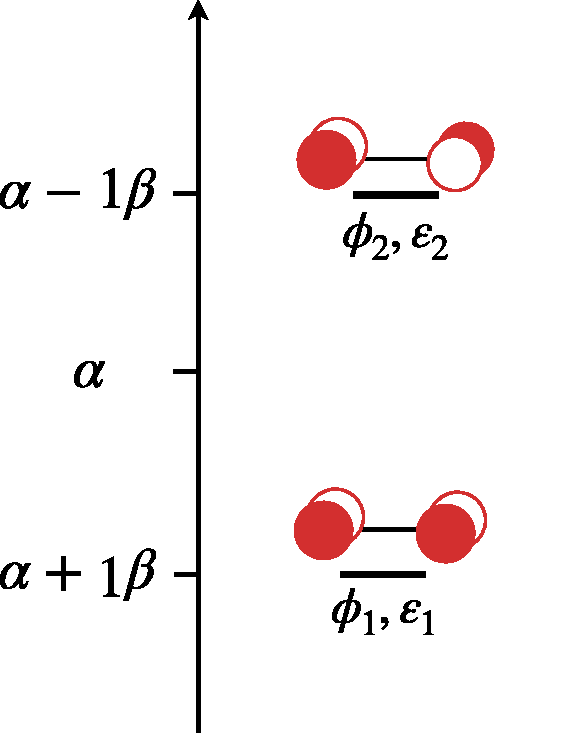
\includegraphics[scale=0.5]{figures/ethylene}
\subsection{Éthylène (sous forme matricielle)}
on peut aussi résoudre sous forme matricielle :
\[\begin{pmatrix}\alpha&\beta\\ \beta &\alpha \end{pmatrix} \begin{pmatrix}c_1\\c_2 \end{pmatrix} = \epsilon \begin{pmatrix}c_1\\c_2 \end{pmatrix}\]

On réécrit  :
\[\begin{pmatrix}\alpha-\epsilon&\beta\\ \beta &\alpha-\epsilon \end{pmatrix} \begin{pmatrix}c_1\\c_2 \end{pmatrix} = \begin{pmatrix}0\\0 \end{pmatrix}\]
En posant \(\frac{\alpha-\epsilon}{\beta} = x\) :
\[\beta \begin{pmatrix}x&1\\ 1 &x \end{pmatrix} \begin{pmatrix}c_1\\c_2 \end{pmatrix} = \begin{pmatrix}0\\0 \end{pmatrix}\]Le déterminant doit \^etre nul donc :
\[x^2-1 = 0\Rightarrow x = \pm 1\] On en déduit que \(\epsilon = \alpha \pm \beta\).

On cherche maintenant les vecteurs propres. On prend \(x = 1\), donc \[\begin{pmatrix}1&1\\1&1\end{pmatrix}\begin{pmatrix}c_1\\c_2 \end{pmatrix} = \begin{pmatrix}0\\0 \end{pmatrix}\]
On en déduit que \(c_1+c_2=0\Rightarrow c_1=-c_2\).

Pour les déterminer, on utilise la condition de normalisation sur \(\phi^+ = c_1(\chi_1+\chi_2)\) : \[\langle \phi^+|\phi^+\rangle = c_1^2(\langle \chi_1|\chi_1\rangle-\langle \chi_1|\chi_2\rangle+\langle \chi_2|\chi_2\rangle-\langle \chi_1|\chi_2\rangle) = c_1^2\times 2 \Rightarrow c_1 = \pm \frac{1}{\sqrt{2}}\]
\warningInfo{Différence}{Par rapport à la diagonalisation complète, on remarque ici que l'énergie de stabilisation et de déstabilisation \(\beta\) sont les m\^emes, ce qui n'est pas le cas dans la méthode exacte}

\subsection{H3 trigonal}
Les 3 atomes d'hydrogène sont liés entre eux : c'est une strycture cyclique. Il faut donc trouver le déterminant de \[\begin{vmatrix}
x&1&1\\
1&x&1\\
1&1&x
\end{vmatrix} = (x-1)^2(x+2)\] On remarque qu'il y a une racine double. Il y aura donc 2 OM dégénérées au niveau d'énergie \(\alpha-1\beta\).
\warningInfo{Multiplicité des racines}{La Multiplicité d'une racine donne le nombre d'OA ayant le m\^eme niveau d'énergie. }
Commençons par l'OM du niveau \(\alpha+2\beta\) en replaçant \(x\) par sa valeur \(-2\). On a le système \[\left\{\begin{matrix}
-2c_1+c_2+c_3=0\\
c_1-2c_2+c_3=0\\
c_1+c_2-2c_3=0
\end{matrix}\right.\] qui donne \(c_1=c_2=c_3\)\marginInfo{On peut déjà remarquer que les OA de l'OM seront de m\^eme taille car les coefficients sont égaux}. On applique la condition de normalisation sur \(\phi_1 = c_1(\chi_1+\chi_2+\chi_3)\) pour trouver \(c_1 = \pm \frac{1}{\sqrt{3}}\).

Trouvons maintenant \(\phi_2\), une des OM dégénérées du niveau \(\alpha-1\beta\). La résolution du système conduit à \(c_1+c_2+c_3 =0\). Comme on est en présence d'OM dégénérées, on peut mettre un coefficient à nul, ici on choisit \(c_1 = 0\). On obtient ainsi \(c_2=-c_3\). On a ainsi \[\phi_2 = c_2(\chi_2-\chi_3)\]La conditon de normalisation donne \(c_2 = \pm \frac{1}{\sqrt{2}}\).

Pour trouver la seconde OM dégénérée, on ne peut pas mettre \(c_2\) ou \(c_3\) à 0 car on trouverait la m\^eme OM. On va utiliser la propriété d'orthogonalité des OM avec \(\phi_2\) et \(\phi_1\).


\begin{align*}
\langle \phi_3 | \phi_2 \rangle &= \left\langle \pm \frac{1}{\sqrt{2}}(\chi_2 - \chi_3) \bigg| c_1\chi_1 + c_2\chi_2 + c_3\chi_3 \right\rangle \\
&= \pm \frac{1}{\sqrt{2}} \left[ c_1\langle\chi_2|\chi_1\rangle + c_2\langle\chi_2|\chi_2\rangle + c_3\langle\chi_2|\chi_3\rangle - c_1\langle\chi_3|\chi_1\rangle - c_2\langle\chi_3|\chi_2\rangle - c_3\langle\chi_3|\chi_3\rangle \right] \\
&= \pm \frac{1}{\sqrt{2}} \left[ c_1(0) + c_2(1) + c_3(0) - c_1(0) - c_2(0) - c_3(1) \right] \\
&= \pm \frac{1}{\sqrt{2}} (c_2 - c_3)
\end{align*}
La condition est donc $c_2 = c_3$.

Pour la seconde condition d'orthogonalité :

\begin{align*}
\langle \phi_1 | \phi_3 \rangle &= \left\langle \pm \frac{1}{\sqrt{3}}(\chi_1+\chi_2+\chi_3) \bigg| c_1\chi_1+c_2\chi_2+c_2\chi_3 \right\rangle \\
&= \pm \frac{1}{\sqrt{3}} \left[ c_1\langle\chi_1|\chi_1\rangle + c_2\langle\chi_1|\chi_2\rangle + c_2\langle\chi_1|\chi_3\rangle \right. \\
& \quad + \left. c_1\langle\chi_2|\chi_1\rangle + c_2\langle\chi_2|\chi_2\rangle + c_2\langle\chi_2|\chi_3\rangle \right. \\
& \quad + \left. c_1\langle\chi_3|\chi_1\rangle + c_2\langle\chi_3|\chi_2\rangle + c_2\langle\chi_3|\chi_3\rangle \right] \\
&= \pm \frac{1}{\sqrt{3}} \left[ c_1(1) + c_2(1) + c_2(1) \right] \\
&= \pm \frac{1}{\sqrt{3}}(c_1 + 2c_2)
\end{align*}
La condition est donc $c_1 = -2c_2$.


On trouve ainsi \(c_2 = c_3, c_1 = -2c_2\). Avec la condition de normalisation, on obtient \(c_2 = \pm \frac{1}{\sqrt{6}}\)
Donc \[\phi_3 = \pm \frac{1}{\sqrt{6}}(-2\chi_1+\chi_2+\chi_3)\]
%DOM TODO page 74
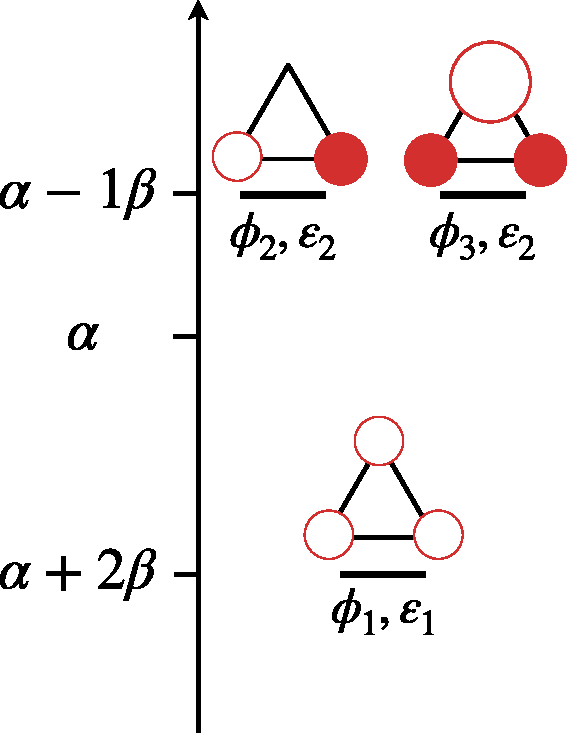
\includegraphics[scale=0.5]{figures/trigo}
\subsubsection{H4 Carré plan}
Le système est \[\begin{pmatrix}
x & 1 & 0 & 1 \\
1 & x & 1 & 0 \\
0 & 1 & x & 1 \\
1 & 0 & 1 & x \\
\end{pmatrix}\begin{pmatrix}c_1\\c_2\\c_3\\c_4 \end{pmatrix} = 0\]
On cherche le déterminant de \[\begin{vmatrix}
x & 1 & 0 & 1 \\
1 & x & 1 & 0 \\
0 & 1 & x & 1 \\
1 & 0 & 1 & x \\
\end{vmatrix}\] On obtient \[x^2(x-2)(x+2)\] On aura donc 2 OA dégénérées au niveau \(\alpha\), une au niveau \(\alpha-2\beta\) et une au niveau \(\alpha+2\beta\)

Cherchons \(\phi_1\) pour \(x=-2\). En injectant dans le système, on trouve \(c_1=c_2=c_3=c_4\). Donc \(\phi_1 = c_1(\chi_1+\chi_2+\chi_3+\chi_4)\). La condition de normalisation donne \(c_1 = \frac{1}{\sqrt{4}}\), donc \[\phi_1 = \pm \frac{1}{2}(\chi_1+\chi_2+\chi_3+\chi_4)\]

Cherchons \(\phi_3\). En injectant \(x=2\), trouve \(c_1=-c_2=c_3=-c_4\). Donc avec la condition de normalisation, on obtient \[\phi_4 = \pm \frac{1}{2}(\chi_1-\chi_2+\chi_3-\chi_4)\]

Cherchons maintenant \(\phi_2\). Avec \(x=0\), on a
\begin{flalign*}
c_2&=-c_4\\
c_1&=-c_3
\end{flalign*}
Les OM sont dégénérées, on peut donc supposer\marginCritical{C'est un choix que l'on fait. Cela respecte la physique car les autres coefficients sont ne sont pas nuls, donc l'OM n'est pas nulle.} \(c_2 = -c_4 = 0\). Ainsi, \(\phi_1 = c_1(\chi_1-\chi_3)\). Finalement \[\phi_2 = \pm \frac{1}{\sqrt{2}}(\chi_1-\chi_3)\]

Pour la dernière, on a \(\phi_3 = c_1\chi_1+c_2\chi_2-c_1\chi_3-c_2\chi_4\). On se sert de la condition d'orthogonalité avec \(\phi_2\) :

\begin{align*}
\langle \phi_2 | \phi_3 \rangle &= \left\langle \pm \frac{1}{\sqrt{2}}(\chi_1-\chi_3) \bigg| c_1\chi_1+c_2\chi_2-c_1\chi_3-c_2\chi_4 \right\rangle \\
&= \pm \frac{1}{\sqrt{2}} \left[ c_1\langle\chi_1|\chi_1\rangle + c_2\langle\chi_1|\chi_2\rangle - c_1\langle\chi_1|\chi_3\rangle - c_2\langle\chi_1|\chi_4\rangle \right. \\
& \quad - \left. c_1\langle\chi_3|\chi_1\rangle - c_2\langle\chi_3|\chi_2\rangle - (-c_1)\langle\chi_3|\chi_3\rangle - (-c_2)\langle\chi_3|\chi_4\rangle \right] \\
&= \pm \frac{1}{\sqrt{2}} [ c_1(1) - (-c_1)(1) ] \\
&= \pm \frac{1}{\sqrt{2}}(c_1+c_1) \\
&= \pm \frac{1}{\sqrt{2}}(2c_1) \\
&= \pm \sqrt{2}c_1
\end{align*}
La condition est donc $c_1 = 0$. Avec la condition de normalisation, on a \[\phi_3 = \pm \frac{1}{\sqrt{2}}(\chi_2-\chi_4)\]

\includegraphics[scale=0.5]{figures/carre_plan}

On aurait pu trouver le m\^eme DOM avec la méthode des fragments et en coupant la molécule à 45°.
\subsection{H4 Tétraédrique}
Dans un tétraèdre régulier, chaque atome est lié aux trois autres.

\paragraph{1. Déterminant}
En posant $x = \frac{\alpha-\epsilon}{\beta}$, le système s'écrit :
\[
\begin{vmatrix}
x & 1 & 1 & 1 \\
1 & x & 1 & 1 \\
1 & 1 & x & 1 \\
1 & 1 & 1 & x \\
\end{vmatrix} = 0
\]
Le développement de ce déterminant conduit au polynôme caractéristique :
\[ (x-3)(x+1)^3 = 0 \]

\paragraph{2. Niveaux d'énergie}
Les racines sont $x_1 = 3$ et une racine triple $x_{2,3,4} = -1$. En utilisant $\epsilon = \alpha - x\beta$, on obtient :
\begin{itemize}
    \item $\epsilon_1 = \alpha + 3\beta$ (Niveau liant, non dégénéré)
    \item $\epsilon_{2,3,4} = \alpha - \beta$ (Niveau antiliant, triplement dégénéré)
\end{itemize}

\paragraph{3. Calcul des Orbitales Moléculaires (OM)}

\textbf{OM Fondamentale $\phi_1$ ($x = -3$)} :

Par symétrie, tous les coefficients sont égaux ($c_1=c_2=c_3=c_4$). La condition de normalisation $\sum c_i^2 = 1$ donne :
\[ 4c_1^2 = 1 \Rightarrow c_1 = \frac{1}{2} \]
\[ \phi_1 = \frac{1}{2}(\chi_1 + \chi_2 + \chi_3 + \chi_4) \]

\textbf{OMs Dégénérées $\phi_2, \phi_3, \phi_4$ ($x = 1$)} :

Le système se réduit à la condition unique : $c_1 + c_2 + c_3 + c_4 = 0$. Comme le niveau est triplement dégénéré, on construit des combinaisons orthogonales :

\begin{itemize}
    \item \textbf{Pour $\phi_2$} : On choisit $c_3 = c_4 = 0$\marginTips{En effet, c'est notre première OM dégénérée. On a donc seulement l' équation du système pour résoudre le système et la normalisation. Il faut n'avoir que 2 inconnues pour résoudre le système. On va donc poser pour simplifier $c_3 = c_4 = 0$}. Alors $c_1 + c_2 = 0 \Rightarrow c_1 = -c_2$.
    Après normalisation ($2c_1^2 = 1$) :
    \[ \phi_2 = \frac{1}{\sqrt{2}}(\chi_1 - \chi_2) \]

    \item \textbf{Pour $\phi_3$} : On cherche une fonction orthogonale à $\phi_1$ et $\phi_2$.

    On impose $c_4 = 0$\marginTips{En effet, c'est deuxième  OM dégénérée. On a donc l'équation du système pour résoudre le système, l'orthogonalité avec la première OM et la normalisation. Il faut n'avoir que 3 inconnues pour résoudre le système. On va donc poser pour simplifier $c_4 = 0$}.

    L'orthogonalité avec $\phi_2$ impose $c_1 = c_2$.

    La condition $c_1+c_2+c_3=0$ devient $2c_1 + c_3 = 0$.

    Après normalisation ($c_1^2 + c_1^2 + (-2c_1)^2 = 1 \Rightarrow 6c_1^2 = 1$) :
    \[ \phi_3 = \frac{1}{\sqrt{6}}(\chi_1 + \chi_2 - 2\chi_3) \]

    \item \textbf{Pour $\phi_4$} : Par orthogonalité avec les trois précédentes, on déduit la dernière combinaison :
    \[ \phi_4 = \frac{1}{\sqrt{12}}(\chi_1 + \chi_2 + \chi_3 - 3\chi_4) \]
\end{itemize}
 \end{document}
